\documentclass[12pt, a4paper]{article}

% ----- Package Imports -----
\usepackage[utf8]{inputenc}                % UTF-8 encoding
\usepackage[T1]{fontenc}                   % Output font encoding
\usepackage{mathpazo}                      % Palatino font for text and math
\usepackage{amsmath, amssymb, amsthm}        % Mathematics packages
\usepackage{graphicx}                      % Graphics inclusion
\usepackage{float}                         % Improved float handling
\usepackage{caption}                       % Custom captions
\usepackage{subcaption}                    % Subfigures
\usepackage{hyperref}                      % Hyperlinks
\usepackage[numbers]{natbib}               % Numerical citations
\usepackage{xcolor}                        % Color definitions
\usepackage{microtype}                     % Improved typography
\usepackage{setspace}                      % Line spacing
\usepackage{fancyhdr}                      % Custom headers and footers
\usepackage{titlesec}                      % Custom section titles
\usepackage{booktabs}                      % Enhanced tables
\usepackage{enumitem}                      % Customized lists
\usepackage{algorithm}                     % Algorithms
\usepackage{algpseudocode}                 % Pseudocode
\usepackage{mathtools}                     % Enhanced math features
\usepackage{geometry}                      % Page layout
\usepackage{doi}                           % DOI links in bibliography

% ----- Figures configuration -----
\graphicspath{{figures/}}                  % Path to figures
\captionsetup{font=small, labelfont=bf}     % Caption settings
\captionsetup[sub]{font=small}             % Subcaption settings

% ----- Page Layout -----
\geometry{
    a4paper,
    left=1in,
    right=1in,
    top=1in,
    bottom=1in,
}

% ----- Typography and Spacing -----
\microtypesetup{protrusion=true, expansion=true}  % Microtype settings
\setstretch{1.5}                                 % Line spacing set to 1.5

% ----- Custom Colors -----
\definecolor{accentred}{RGB}{204, 0, 0}
\definecolor{accentblue}{RGB}{0, 102, 204}
\definecolor{accentgreen}{RGB}{0, 153, 0}
\definecolor{lightgray}{RGB}{240, 240, 240}

% ----- Hyperlink Configuration -----
\hypersetup{
    colorlinks=true,
    linkcolor=accentblue,       % Internal links (sections, etc.)
    citecolor=accentgreen,      % Citation links
    urlcolor=accentred,         % External URLs
    linktoc=all,                % Links include both text and page number in TOC
    pdfauthor={Your Name},
    pdftitle={Fluid-Structure Interaction Analysis of Pulsatile Flow in Arterial Aneurysms with Physics-Informed Neural Networks and Computational Fluid Dynamics},
    pdfsubject={Research Paper},
}

% ----- Header and Footer Configuration -----
\pagestyle{fancy}
\fancyhf{}  % Clear all header and footer fields
\fancyhead[L]{\nouppercase{\leftmark}}  % Left header: section title
\fancyhead[R]{\thepage}                 % Right header: page number
\renewcommand{\headrulewidth}{0.5pt}    % Header rule
\renewcommand{\footrulewidth}{0pt}      % No footer rule

% ----- Section Title Configuration -----
\titleformat{\section}
  {\normalfont\Large\bfseries\color{accentblue}}{\thesection}{1em}{}
\titleformat{\subsection}
  {\normalfont\large\bfseries\color{accentgreen}}{\thesubsection}{1em}{}
\titleformat{\subsubsection}
  {\normalfont\normalsize\bfseries\color{accentgreen}}{\thesubsubsection}{1em}{}

% ----- Title and Author -----
\title{
    \vspace{-2cm} % Adjust vertical spacing as needed
    \large \textbf{Fluid-Structure Interaction Analysis of Pulsatile Flow in Arterial Aneurysms with Physics-Informed Neural Networks and Computational Fluid Dynamics}\\
}

\author{
    Michael Ajao-Olarinoye\textsuperscript{1} \\
    \textsuperscript{1}Center for Computational Science and Mathematical Modelling \\
    \texttt{olarinoyem@coventry.ac.uk}
}

\date{}

\begin{document}

\maketitle

%\begin{abstract}
%    \noindent
%    This study presents a comprehensive analysis of fluid-structure interactions (FSI) in pulsatile arterial aneurysms using a hybrid approach combining Physics-Informed Neural Networks (PINNs) and Computational Fluid Dynamics (CFD). PINNs incorporate the governing physical laws directly into the loss function, thereby reducing data requirements and computational costs. The methodology is validated against CFD data, demonstrating its potential for rapid, high-resolution hemodynamic analyses. 
%\end{abstract}

\section{Physics-Informed Neural Networks}
\label{sec:PINNs}

\subsection{Overview}
\label{sec:PINN_Overview}
High-fidelity Computational Fluid Dynamics (CFD) simulations (Section~2.4) offer detailed insights into arterial hemodynamics but are computationally expensive and require significant expertise in mesh generation, solver tuning, and post-processing. In contrast, Physics-Informed Neural Networks (PINNs)~\citep{raissi2019physics} combine deep learning with physics-based modeling by embedding the governing partial differential equations (PDEs) directly into the network's loss function. This integration enables the network to learn realistic flow solutions while significantly reducing the need for extensive CFD re-runs when parameters or geometries change.

By incorporating PDE residuals and boundary conditions into the training process, PINNs naturally enforce physical constraints, reduce overfitting, and require fewer labeled data points. Consequently, PINNs can complement or even partially replace traditional CFD simulations, offering:
\begin{enumerate}[label=\arabic*)]
    \item \textbf{Denser solution fields:} PINNs can be evaluated at arbitrary spatial and temporal points, yielding high-resolution predictions that surpass the original CFD mesh density.
    \item \textbf{Enhanced generalization:} Adaptation to new boundary conditions or geometrical changes is possible with minimal retraining.
    \item \textbf{Reduced computational cost:} Once trained, PINN inference is rapid, making real-time or iterative analyses feasible.
\end{enumerate}
In this study, we integrate PINNs with CFD data to predict pressure, velocity components, and wall shear stress (WSS) in both healthy and Marfan Syndrome aortic models (Section~2.1), enabling a direct comparison of flow patterns and shear forces between non-pathological and aneurysmal vessels.

\subsection{Formulation of Physics-Informed Neural Networks}
\label{sec:PINN_Formulation}

Modeling pulsatile flow in arterial segments requires that the continuity and momentum conservation equations be enforced to capture the essential hemodynamic effects. In our study, the blood flow model and associated boundary conditions are described in Sections~2.2 and 2.3 using the Reynolds-averaged Navier–Stokes (RANS) equations (Equations (2.1)–(2.9)). Let \(\mathbf{u} = (u,v,w)\) denote the velocity field, \(p\) the pressure, \(\rho\) the fluid density, and \(\mu\) the dynamic viscosity. The continuity and momentum equations are combined into the Navier–Stokes system, which governs the evolution of the velocity field and pressure in response to external forces and viscous effects.

In standard index notation (with the Einstein summation convention), the governing equations are written as
\[
\begin{aligned}
\frac{\partial u_i}{\partial x_i} &= 0, \\
\rho\left(\frac{\partial u_i}{\partial t} + u_j\,\frac{\partial u_i}{\partial x_j}\right) &= -\frac{\partial p}{\partial x_i} + \mu\,\frac{\partial^2 u_i}{\partial x_j^2},
\end{aligned}
\tag{3.1}
\]
where \(i,\,j=1,2,3\) correspond to the spatial coordinates. Equation (3.1) thus encapsulates both the continuity equation (first line) and the momentum (Navier–Stokes) equation (second line).

The boundary conditions are as follows:
\begin{itemize}
    \item A no-slip condition on the arterial walls, i.e., \(\mathbf{u} = \mathbf{0}\) on the wall boundary,
    \item Zero relative pressure at the outlet, and
    \item A pulsatile inlet velocity prescribed on the inlet boundary.
\end{itemize}
In our formulation, these conditions are enforced via penalty terms in the loss function. For example, the no-slip and inlet conditions are imposed as
\[
L_{\mathrm{boundary}} = \Bigl\|\mathbf{u}\Big|_{\partial\Omega_{\mathrm{wall}}} - \mathbf{0}\Bigr\|_2, \quad
L_{\mathrm{inlet}} = \Bigl\|\mathbf{u}\Big|_{\partial\Omega_{\mathrm{inlet}}} - \mathbf{u}_{\mathrm{inlet}}(t)\Bigr\|_2,
\]
where \(\partial\Omega_{\mathrm{wall}}\) and \(\partial\Omega_{\mathrm{inlet}}\) denote the vessel wall and inlet boundaries, respectively.

Within the PINN framework, neural networks are used to approximate the functions
\[
u(x,y,z,t),\quad v(x,y,z,t),\quad w(x,y,z,t),\quad p(x,y,z,t),
\]
as well as the three wall shear stress (WSS) components
\[
\tau_x(x,y,z,t),\quad \tau_y(x,y,z,t),\quad \tau_z(x,y,z,t).
\]
Together, these functions capture the spatiotemporal evolution of blood flow and the shear forces acting on the vessel walls.

Let \(F(\cdot)\) represent the nonlinear operator corresponding to the Navier–Stokes system. The physics residual loss is then defined as
\[
L_{\mathrm{physics}} = \Bigl\|F(\mathbf{u},p)\Bigr\|_2,
\]
where \(\|\cdot\|_2\) denotes the Euclidean norm. Minimizing this loss term drives the network to produce solutions that are consistent with the Navier–Stokes and continuity equations, even in regions where direct measurements are not available.

Furthermore, when CFD reference data (e.g., \(\mathbf{u}_{\mathrm{CFD}}\), \(p_{\mathrm{CFD}}\), and \(\boldsymbol{\tau}_{\mathrm{CFD}}\)) are available, a data-fitting loss is incorporated:
\[
L_{\mathrm{data}} = \Bigl\|\mathbf{u}_{\mathrm{NN}} - \mathbf{u}_{\mathrm{CFD}}\Bigr\|_2 + \Bigl\|p_{\mathrm{NN}} - p_{\mathrm{CFD}}\Bigr\|_2 + \Bigl\|\boldsymbol{\tau}_{\mathrm{NN}} - \boldsymbol{\tau}_{\mathrm{CFD}}\Bigr\|_2.
\]
The total loss function is then expressed as
\begin{equation}
L_{total} = \lambda_{\mathrm{physics}}\,L_{\mathrm{physics}} + \lambda_{\mathrm{boundary}}\,L_{\mathrm{boundary}} + \lambda_{\mathrm{inlet}}\,L_{\mathrm{inlet}} + \lambda_{\mathrm{data}}\,L_{\mathrm{data}},
\label{eq:total_loss}
\end{equation}
where \(\lambda_{\mathrm{physics}}, \lambda_{\mathrm{boundary}}, \lambda_{\mathrm{inlet}}, \lambda_{\mathrm{data}}\) are self-adaptive weighting coefficients that are optimized during training to balance the contributions of each loss component~\citep{mcclenny2020self}. The details of the self-adaptive weighting mechanism are discussed in Section~\ref{sec:self_adaptive_weighting}.


% \begin{equation}
% \nabla \cdot \mathbf{u} = 0, 
% \quad
% \rho \frac{\partial \mathbf{u}}{\partial t} + \rho (\mathbf{u} \cdot \nabla)\mathbf{u}
% = -\nabla p + \mu \nabla^2 \mathbf{u}.
% \label{eq:navier_stokes}
% \end{equation}

% \begin{equation}
% \begin{split}
% \frac{\partial u_i}{\partial x_i} &= 0, \\
% \rho\left(\frac{\partial u_i}{\partial t} + u_j \frac{\partial u_i}{\partial x_j}\right)
% &= -\frac{\partial p}{\partial x_i} + \mu\,\frac{\partial^2 u_i}{\partial x_j^2},
% \end{split}
% \label{eq:navier_stokes}
% \end{equation}

% where the Einstein summation convention is assumed over repeated indices (i.e., \(i,j = 1,2,3\)). \ref{eq:navier_stokes} represents the continuity equation (first line) and the momentum (Navier–Stokes) equation (second line) in a compact, standard format. The continuity equation enforces mass conservation, while the momentum equation describes the balance between pressure gradients, viscous forces, and inertial effects. These equations are supplemented by appropriate boundary conditions and inlet profiles to fully characterize the flow field within the arterial domain.

% The boundary conditions involve a no-slip condition on the arterial walls \((\mathbf{u}=\mathbf{0} \text{ on } \partial\Omega_{\text{wall}})\), zero relative pressure at the outlet, and a pulsatile inlet velocity on \(\partial\Omega_{\text{inlet}}\) (Section~2.3). These boundary and inlet constraints are incorporated into the Physics-Informed Neural Network through penalty terms in the loss function, thereby enforcing consistency between the network’s predictions and the specified physical conditions. Temporal dependence is explicitly modelled to reflect the transient nature of blood flow.


\subsection{Formulation of Physics-Informed Neural Networks}
\label{sec:PINN_Formulation}

Modeling pulsatile flow in arterial segments requires enforcing the fundamental laws of fluid mechanics—namely, the continuity and Navier–Stokes equations—to capture the essential hemodynamic effects. In our study, the blood flow in aortic geometries is modeled using the Reynolds-averaged Navier–Stokes (RANS) framework (see Sections~2.2 and 2.3). Let \(\mathbf{u} = (u,v,w)\) denote the velocity field, \(p\) the pressure, \(\rho\) the fluid density, and \(\mu\) the dynamic viscosity. The Navier–Stokes system, which governs the evolution of the velocity field and pressure under the influence of external forces and viscous effects, is expressed in standard index notation as

\[
\begin{aligned}
\frac{\partial u_i}{\partial x_i} &= 0, \\
\rho\left(\frac{\partial u_i}{\partial t} + u_j\,\frac{\partial u_i}{\partial x_j}\right) &= -\frac{\partial p}{\partial x_i} + \mu\,\frac{\partial^2 u_i}{\partial x_j^2},
\end{aligned}
\tag{3.1}
\]

where the Einstein summation convention is assumed (i.e., summing over repeated indices \(i,j = 1,2,3\)). In our simulations (Sections~2.2 and 2.3), the boundary conditions are prescribed as follows: a no-slip condition on the arterial walls (i.e., \(\mathbf{u} = \mathbf{0}\) on the wall boundary), zero relative pressure at the outlet, and a pulsatile inlet velocity on the inlet boundary. These conditions are incorporated into the PINN framework through penalty terms within the loss function, thereby ensuring that the network’s predictions remain consistent with the physical constraints and the transient nature of blood flow.

Within the PINN framework, the neural network approximates the functions
\[
u(x,y,z,t),\quad v(x,y,z,t),\quad w(x,y,z,t),\quad p(x,y,z,t),
\]
as well as the three wall shear stress (WSS) components
\[
\tau_x(x,y,z,t),\quad \tau_y(x,y,z,t),\quad \tau_z(x,y,z,t).
\]
Together, these variables capture the spatiotemporal evolution of blood flow and the shear forces acting on the vessel walls.

Let \(F(\cdot)\) denote the nonlinear operator corresponding to the Navier–Stokes system defined in Equation (3.1). The physics residual loss is defined as
\[
L_{\mathrm{physics}} = \Bigl\|F(\mathbf{u},p)\Bigr\|_2,
\]
where \(\|\cdot\|_2\) denotes the Euclidean norm. Minimizing this term drives the network to learn solutions that are consistent with the governing equations even in regions where direct data are sparse.

Additionally, the boundary and inlet conditions are enforced via penalty terms:
\[
L_{\mathrm{boundary}} = \Bigl\|\mathbf{u}\Big|_{\partial\Omega_{\mathrm{wall}}} - \mathbf{0}\Bigr\|_2, \quad
L_{\mathrm{inlet}} = \Bigl\|\mathbf{u}\Big|_{\partial\Omega_{\mathrm{inlet}}} - \mathbf{u}_{\mathrm{inlet}}(t)\Bigr\|_2,
\]
where \(\partial\Omega_{\mathrm{wall}}\) and \(\partial\Omega_{\mathrm{inlet}}\) denote the wall and inlet boundaries, respectively, and \(\mathbf{u}_{\mathrm{inlet}}(t)\) is the prescribed pulsatile inlet velocity profile (Section~2.3). When available, CFD reference data for pressure, velocity, and WSS—denoted by \(\mathbf{u}_{\mathrm{CFD}},\,p_{\mathrm{CFD}}\), and \(\boldsymbol{\tau}_{\mathrm{CFD}}\)—are used to define a data-fitting loss:
\[
L_{\mathrm{data}} = \Bigl\|\mathbf{u}_{\mathrm{NN}} - \mathbf{u}_{\mathrm{CFD}}\Bigr\|_2 + \Bigl\|p_{\mathrm{NN}} - p_{\mathrm{CFD}}\Bigr\|_2 + \Bigl\|\boldsymbol{\tau}_{\mathrm{NN}} - \boldsymbol{\tau}_{\mathrm{CFD}}\Bigr\|_2.
\]
Here, the subscripts “NN” and “CFD” denote the PINN predictions and the CFD reference values, respectively.

The total loss function, which combines the physics residual, boundary, inlet, and data-fitting terms, is then given by
\[
L_{total} = \lambda_{\mathrm{physics}}\,L_{\mathrm{physics}} + \lambda_{\mathrm{boundary}}\,L_{\mathrm{boundary}} + \lambda_{\mathrm{inlet}}\,L_{\mathrm{inlet}} + \lambda_{\mathrm{data}}\,L_{\mathrm{data}},
\tag{3.2}
\]
where the weighting coefficients \(\lambda_{\mathrm{physics}}, \lambda_{\mathrm{boundary}}, \lambda_{\mathrm{inlet}}, \lambda_{\mathrm{data}}\) are determined via a self-adaptive scheme \citep{mcclenny2020self} to automatically balance the contributions of each term during training.



\subsection{Formulation of PINNs}
\section{Physics-Informed Neural Networks (PINNs)}
\label{sec:PINNs}

Although high-fidelity CFD simulations provide accurate haemodynamic predictions,
they often incur a high computational cost. To address this limitation, we employ
\emph{Physics-Informed Neural Networks} (PINNs), which embed the governing fluid
equations (Navier--Stokes, continuity, turbulence closure) and boundary conditions
directly into a neural-network loss function. In doing so, PINNs can learn
accurate velocity, pressure, and wall shear stress distributions without relying
exclusively on large, labeled datasets. Instead, the PDEs themselves act as
guiding constraints in the training process.

\subsection{PINN Framework and Motivation}
\label{sec:PINN_Framework}

A PINN can be viewed as a neural network that takes the spatiotemporal
coordinates, \(\bigl(x,y,z,t\bigr)\), as inputs and outputs an approximation to
the relevant flow fields. In this study, the network separately predicts
\begin{itemize}
    \item Pressure, \(p(x,y,z,t)\),
    \item Velocity components, \(\bigl(u,v,w\bigr)(x,y,z,t)\),
    \item Wall shear stress (WSS) components, \(\bigl(\tau_x,\tau_y,\tau_z\bigr)(x,y,z,t)\).
\end{itemize}
Unlike conventional machine-learning models, PINNs penalize deviations from
both \emph{physical laws} and \emph{observed data}, creating a hybrid loss
function. This approach allows the model to exploit fundamental conservation
principles---such as incompressibility and momentum transport---even in
regions where direct data (e.g.\ from simulations or experiments) may be sparse.

\subsection{Constructing the PINN Loss Function}
\label{sec:PINN_Loss}

In our code, the overall PINN loss is composed of four main terms:
\[
L_{\mathrm{total}} 
\;=\;
\lambda_{\mathrm{physics}}\;L_{\mathrm{physics}}
\;+\;
\lambda_{\mathrm{boundary}}\;L_{\mathrm{boundary}}
\;+\;
\lambda_{\mathrm{inlet}}\;L_{\mathrm{inlet}}
\;+\;
\lambda_{\mathrm{data}}\;L_{\mathrm{data}},
\]
where \(\lambda_{\mathrm{physics}}, \lambda_{\mathrm{boundary}}, 
\lambda_{\mathrm{inlet}}, \lambda_{\mathrm{data}}\) are 
\emph{self-adaptive weights} learned during training. The sub-terms are defined
as follows.

\paragraph{1. Physics Residual Loss (\(L_{\mathrm{physics}}\)).}
This term enforces the Navier--Stokes and continuity equations, ensuring that the
neural-network predictions respect conservation of mass and momentum. Formally,
the code computes residuals by differentiating the neural-network outputs
\((u,\,v,\,w,\,p)\) with respect to \(\bigl(x,y,z,t\bigr)\) and substituting these
derivatives into the PDEs. Any deviation from zero is penalized via a Mean
Squared Error (MSE) objective.

\paragraph{2. Boundary Condition Loss (\(L_{\mathrm{boundary}}\)).}
Because we impose a no-slip condition on arterial walls, points identified as
``wall boundary” in the dataset must have \(\bigl(u,v,w\bigr)=\mathbf{0}\). In the
code, a small tolerance is used to detect boundary points, and any non-zero values
at these locations are penalized in the loss.

\paragraph{3. Inlet Condition Loss (\(L_{\mathrm{inlet}}\)).}
A time-varying pulsatile profile is prescribed at the inlet boundary
(Section~\ref{sec:BloodFlowModel}). The PINN enforces this condition by comparing
predicted velocities at inlet points to the known sinusoidal (or piecewise) function.
Any mismatch is penalized to ensure the model reproduces the correct pulsatile
flow.

\paragraph{4. Data-Fitting Loss (\(L_{\mathrm{data}}\)).}
Wherever reference data exist (from CFD or experiments), the network
predictions---\(\bigl(p_{\mathrm{NN}}, \mathbf{u}_{\mathrm{NN}},
\tau_{\mathrm{NN}}\bigr)\)---are matched to the known values,
\(\bigl(p_{\mathrm{CFD}}, \mathbf{u}_{\mathrm{CFD}},
\tau_{\mathrm{CFD}}\bigr)\). The MSE of these differences constitutes
\(L_{\mathrm{data}}\). This ensures that the PINN conforms to any available,
high-fidelity information.

\subsection{Self-Adaptive Weighting}
\label{sec:SelfAdaptive}

One innovative feature of this setup is that the four weighting coefficients
\(\lambda_{\mathrm{physics}}, \lambda_{\mathrm{boundary}}, 
\lambda_{\mathrm{inlet}}, \lambda_{\mathrm{data}}\) are \emph{learnable
parameters}. Rather than fixing them manually, each weight is stored in the code
as \(\log \lambda\), which the model updates during backpropagation. This
technique, known as \emph{self-adaptive loss balancing}~\citep{mcclenny2020self},
helps the training process converge more robustly. Early in training, the network
may focus on satisfying the easier constraints (e.g.\ data-fitting), then gradually
allocate more effort to meeting the stricter PDE requirements, or vice versa, as
needed.

\subsection{PINN Training Workflow}
\label{sec:PINN_Training}

\begin{enumerate}
  \item \textbf{Coordinate and Data Preparation:}
    The inputs, \(\bigl(x,y,z,t\bigr)\), are prepared in PyTorch tensors with
    \texttt{requires\_grad=True} so that automatic differentiation can compute
    partial derivatives for the PDE residuals. The velocity, pressure, and WSS data
    are similarly loaded for supervised matching where available.
  \item \textbf{Forward Pass:} 
    Each specialized PINN (for \(p\), \(u\), \(v\), \(w\), \(\tau_x\), \(\tau_y\), \(\tau_z\))
    takes the input coordinates and returns its predicted field variable. 
    \texttt{torch.autograd.grad} then computes spatial and temporal gradients
    used in the physics loss.
  \item \textbf{Loss Computation:}
    - \(L_{\mathrm{physics}}\) is calculated by inserting the predicted fields 
      into the continuity and momentum equations.
    - \(L_{\mathrm{boundary}}\) checks velocity at boundary points.
    - \(L_{\mathrm{inlet}}\) enforces the inlet velocity profile.
    - \(L_{\mathrm{data}}\) matches network outputs to known CFD data.
    These components are combined using the current (learned) values of 
    \(\lambda_{\mathrm{physics}}, \ldots, \lambda_{\mathrm{data}}\).
  \item \textbf{Backpropagation:} 
    The total loss \(L_{\mathrm{total}}\) is backpropagated to update both the
    PINN’s network weights (which define how it approximates the fields) and the
    log-weights for the self-adaptive coefficients.
  \item \textbf{Convergence and Early Stopping:}
    Training continues until a defined convergence criterion or stopping
    tolerance is met, often monitored via a validation set or by observing a
    plateau in the total loss. This is supported by techniques like gradient
    clipping and mixed precision to maintain numerical stability.
\end{enumerate}

\subsection{Advantages and Outlook}

By incorporating physical laws within the loss function, PINNs can learn
flow solutions in regions where no direct data are available. This property
makes them appealing for scenarios in which collecting or storing extensive
CFD results is infeasible. Additionally, once trained, PINNs can operate as
a \emph{surrogate model} for rapid evaluations under varying boundary
conditions, geometry changes, or material properties. In the context of
arterial haemodynamics, this could facilitate near real-time analysis of
aneurysms, blood-flow distributions, or wall stresses, potentially aiding
clinical decision-making.

\paragraph{Summary.}
In essence, PINNs unify traditional data-driven regression with fundamental
conservation principles. Instead of learning from data \emph{alone}, the
network also “learns” from the PDEs, boundary conditions, and the known
inlet/outlet configurations. The subsequent sections detail how our
PINN-based method compares to high-fidelity CFD simulations in predicting
key haemodynamic parameters (velocity, pressure, and WSS) in both healthy
and aneurysmal aortic geometries.


\subsection{Formulation of Physics-Informed Neural Networks}
\label{sec:PINN_Formulation}
Modeling pulsatile flow in arterial segments requires enforcing the continuity and Navier--Stokes equations. Let $\mathbf{u} = (u,v,w)$ denote the velocity field, $p$ the pressure, $\rho$ the fluid density, and $\mu$ the dynamic viscosity. In a conventional (index) notation, these governing equations are expressed as

\[
\begin{aligned}
\frac{\partial u_i}{\partial x_i} &= 0, \\
\rho\left(\frac{\partial u_i}{\partial t} + u_j \frac{\partial u_i}{\partial x_j}\right) &= -\frac{\partial p}{\partial x_i} + \mu\,\frac{\partial^2 u_i}{\partial x_j^2},
\end{aligned}
\tag{3.1}
\]

where the Einstein summation convention is assumed over repeated indices (i.e., \(i,j = 1,2,3\)). Equation (3.1) represents the continuity equation (first line) and the momentum (Navier–Stokes) equation (second line) in a compact, standard format.

Boundary conditions are imposed as follows:
\begin{itemize}
    \item \textbf{No-slip at vessel walls:} \(\mathbf{u} = \mathbf{0}\) on \(\partial\Omega_{\text{wall}}\).
    \item \textbf{Zero relative pressure:} Applied at the outlet.
    \item \textbf{Pulsatile inlet velocity:} A time-dependent profile is prescribed on \(\partial\Omega_{\text{inlet}}\) (Section~2.3).
\end{itemize}
In the PINN framework, the neural network approximates the functions
\[
u(x,y,z,t),\quad v(x,y,z,t),\quad w(x,y,z,t),\quad p(x,y,z,t),
\]
as well as the wall shear stress components
\[
\tau_x(x,y,z,t),\quad \tau_y(x,y,z,t),\quad \tau_z(x,y,z,t).
\]
The physics residual loss $L_{\mathrm{physics}}$ is defined by the deviation from the Navier--Stokes operator:
\[
L_{\mathrm{physics}} = \Bigl\|F(\mathbf{u},p)\Bigr\|_2,
\]
where $F(\cdot)$ represents the left-hand side of Equation (3.1) minus the right-hand side. Additional loss terms enforce the boundary conditions:
\[
L_{\mathrm{boundary}} = \Bigl\|\mathbf{u}\Big|_{\partial\Omega_{\text{wall}}} - \mathbf{0}\Bigr\|_2, \quad
L_{\mathrm{inlet}} = \Bigl\|\mathbf{u}\Big|_{\Gamma_{\mathrm{inlet}}} - \mathbf{u}_{\mathrm{inlet}}(t)\Bigr\|_2.
\]
Furthermore, if CFD reference data $(\mathbf{u}_{\mathrm{CFD}},\,p_{\mathrm{CFD}},\,\tau_{\mathrm{CFD}})$ are available, a data-fitting loss is included:
\[
L_{\mathrm{data}} = \Bigl\|\mathbf{u}_{\mathrm{NN}} - \mathbf{u}_{\mathrm{CFD}}\Bigr\|_2 + \Bigl\|p_{\mathrm{NN}} - p_{\mathrm{CFD}}\Bigr\|_2 + \Bigl\|\tau_{\mathrm{NN}} - \tau_{\mathrm{CFD}}\Bigr\|_2.
\]
Thus, the total loss is given by
\begin{equation}
L_{total} = \lambda_{\mathrm{physics}}\,L_{\mathrm{physics}} + \lambda_{\mathrm{boundary}}\,L_{\mathrm{boundary}} + \lambda_{\mathrm{inlet}}\,L_{\mathrm{inlet}} + \lambda_{\mathrm{data}}\,L_{\mathrm{data}},
\label{eq:total_loss}
\end{equation}
where the weights $\lambda_i$ are determined via a self-adaptive loss weighting scheme (Section~3.3.1).

\subsection{Neural Network Architecture}
\label{sec:PINN_Architecture_Training}
In this study, we train separate PINNs for pressure $p$, velocity components $(u,v,w)$, and the three WSS components $(\tau_x,\tau_y,\tau_z)$, each as a function of space and time $t$. Each network is a fully connected feed-forward architecture with $L=10$ hidden layers and $N=64$ neurons per layer. We employ the Swish activation function~\citep{ramachandran2017searching}, defined as
\[
\mathrm{Swish}(x) = x\,\sigma(\beta x),
\]
where $\sigma(\cdot)$ is the sigmoid function and $\beta$ is a learnable parameter. Batch normalization is applied to each layer to improve stability, and weights are initialized using the Kaiming normal method~\citep{he2015delving}.

\subsubsection{Self-Adaptive Loss Weighting}
\label{sec:self_adaptive_weighting}
Balancing multiple loss components (physics, boundary, inlet, and data) is critical for successful training. To achieve this, we employ a self-adaptive weighting strategy inspired by \citet{mcclenny2020self}. We introduce learnable parameters $\log \lambda_i$ (for $i\in\{\mathrm{phys}, \mathrm{bound}, \mathrm{inlet}, \mathrm{data}\}$) such that
\[
\lambda_i = \exp(\log \lambda_i),
\]
ensuring that the weights remain positive throughout training. These weights are optimized jointly with the network parameters, allowing the model to automatically balance the contributions of the various loss components. Algorithm~\ref{alg:self_adaptive_weighting} outlines this process.

\begin{algorithm}[htbp]
    \caption{Self-Adaptive Loss Weighting in PINNs}
    \label{alg:self_adaptive_weighting}
    \begin{algorithmic}[1]
    \Require Initial network weights $\theta$, initial $\log \lambda_i$, learning rates for $\theta$ and $\log \lambda_i$
    \Ensure Trained network weights $\theta^*$ and optimized $\lambda_i^*$
    \While{not converged}
        \State Sample mini-batch of training points
        \State Forward pass to compute predictions $\mathbf{u}_{\mathrm{NN}}$, $p_{\mathrm{NN}}$, $\boldsymbol{\tau}_{\mathrm{NN}}$
        \State Compute individual loss components:
        \State \quad $\mathcal{L}_{\mathrm{phys}} = \|F(\mathbf{u}_{\mathrm{NN}},p_{\mathrm{NN}})\|_2^2$
        \State \quad $\mathcal{L}_{\mathrm{bound}} = \|\mathbf{u}_{\mathrm{NN}}|_{\partial\Omega_{\mathrm{wall}}} - \mathbf{0}\|_2^2$
        \State \quad $\mathcal{L}_{\mathrm{inlet}} = \|\mathbf{u}_{\mathrm{NN}}|_{\Gamma_{\mathrm{inlet}}} - \mathbf{u}_{\mathrm{inlet}}(t)\|_2^2$
        \State \quad $\mathcal{L}_{\mathrm{data}} = \|\mathbf{u}_{\mathrm{NN}} - \mathbf{u}_{\mathrm{CFD}}\|_2^2 + \|p_{\mathrm{NN}} - p_{\mathrm{CFD}}\|_2^2 + \|\boldsymbol{\tau}_{\mathrm{NN}} - \boldsymbol{\tau}_{\mathrm{CFD}}\|_2^2$
        \State Set $\mathcal{L}_{\mathrm{total}} = \lambda_{\mathrm{phys}}\,\mathcal{L}_{\mathrm{phys}} + \lambda_{\mathrm{bound}}\,\mathcal{L}_{\mathrm{bound}} + \lambda_{\mathrm{inlet}}\,\mathcal{L}_{\mathrm{inlet}} + \lambda_{\mathrm{data}}\,\mathcal{L}_{\mathrm{data}}$
        \State Backpropagate $\mathcal{L}_{\mathrm{total}}$ to compute gradients for $\theta$ and $\log \lambda_i$
        \State Update network weights: $\theta \leftarrow \theta - \eta_\theta \nabla_{\theta}\mathcal{L}_{\mathrm{total}}$
        \State Update log-weights: $\log \lambda_i \leftarrow \log \lambda_i - \eta_\lambda \nabla_{\log \lambda_i}\mathcal{L}_{\mathrm{total}}$
    \EndWhile
    \State \textbf{Return} $\theta^*$, $\lambda_i^*$
    \end{algorithmic}
\end{algorithm}

\subsection{Data Processing and Experimental Setup}
\label{sec:data_processing}
CFD simulation data from healthy (0024 and 0142) and aneurysmal (0021, 0022, 0023, 0025) aortic geometries were obtained for both systolic and diastolic phases. Each dataset includes spatial coordinates (X, Y, Z), time, pressure, velocity (u, v, w), and wall shear stress (τx, τy, τz). The data processing steps were as follows:
\begin{enumerate}
    \item \textbf{Data Cleaning:} Remove incomplete records and verify physical consistency, yielding approximately 11,005 points per time step.
    \item \textbf{Normalization:} Normalize spatial coordinates to the interval \([-1,1]\), time to \([0,1]\) over the cardiac cycle, and each of the physical variables independently using Min--Max scaling.
    \item \textbf{Boundary Identification:} Identify vessel-wall points using a velocity magnitude threshold ($|u|, |v|, |w| < 10^{-5}$) to enforce the no-slip condition.
    \item \textbf{Data Organization:} Organize the data by grouping healthy and aneurysmal cases with uniform time sampling.
    \item \textbf{Quality Control:} Perform checks for consistency in velocity and pressure fields, verify mass conservation at inlet/outlet, and ensure temporal continuity.
\end{enumerate}

\subsection{Point Density Analysis and Spatial Discretization}
A significant advantage of PINNs is the ability to produce mesh-free, continuous predictions of flow variables. Our analysis of the training dataset confirmed that 11,005 points provide uniform spatial coverage and sufficient resolution to capture the complex flow features in both healthy and aneurysmal geometries. Furthermore, once trained, the PINN can generate predictions at a density approximately 100.5 times higher (over 1,100,000 points) while maintaining rapid inference speeds.

Figure~\ref{fig:mesh_analysis} displays the 2D projections of the training point distribution, while Figure~\ref{fig:density_comparison} compares the original CFD point distribution with the high-resolution PINN predictions and illustrates the computational time benefits of the PINN approach.

\begin{figure}[htbp]
    \centering
    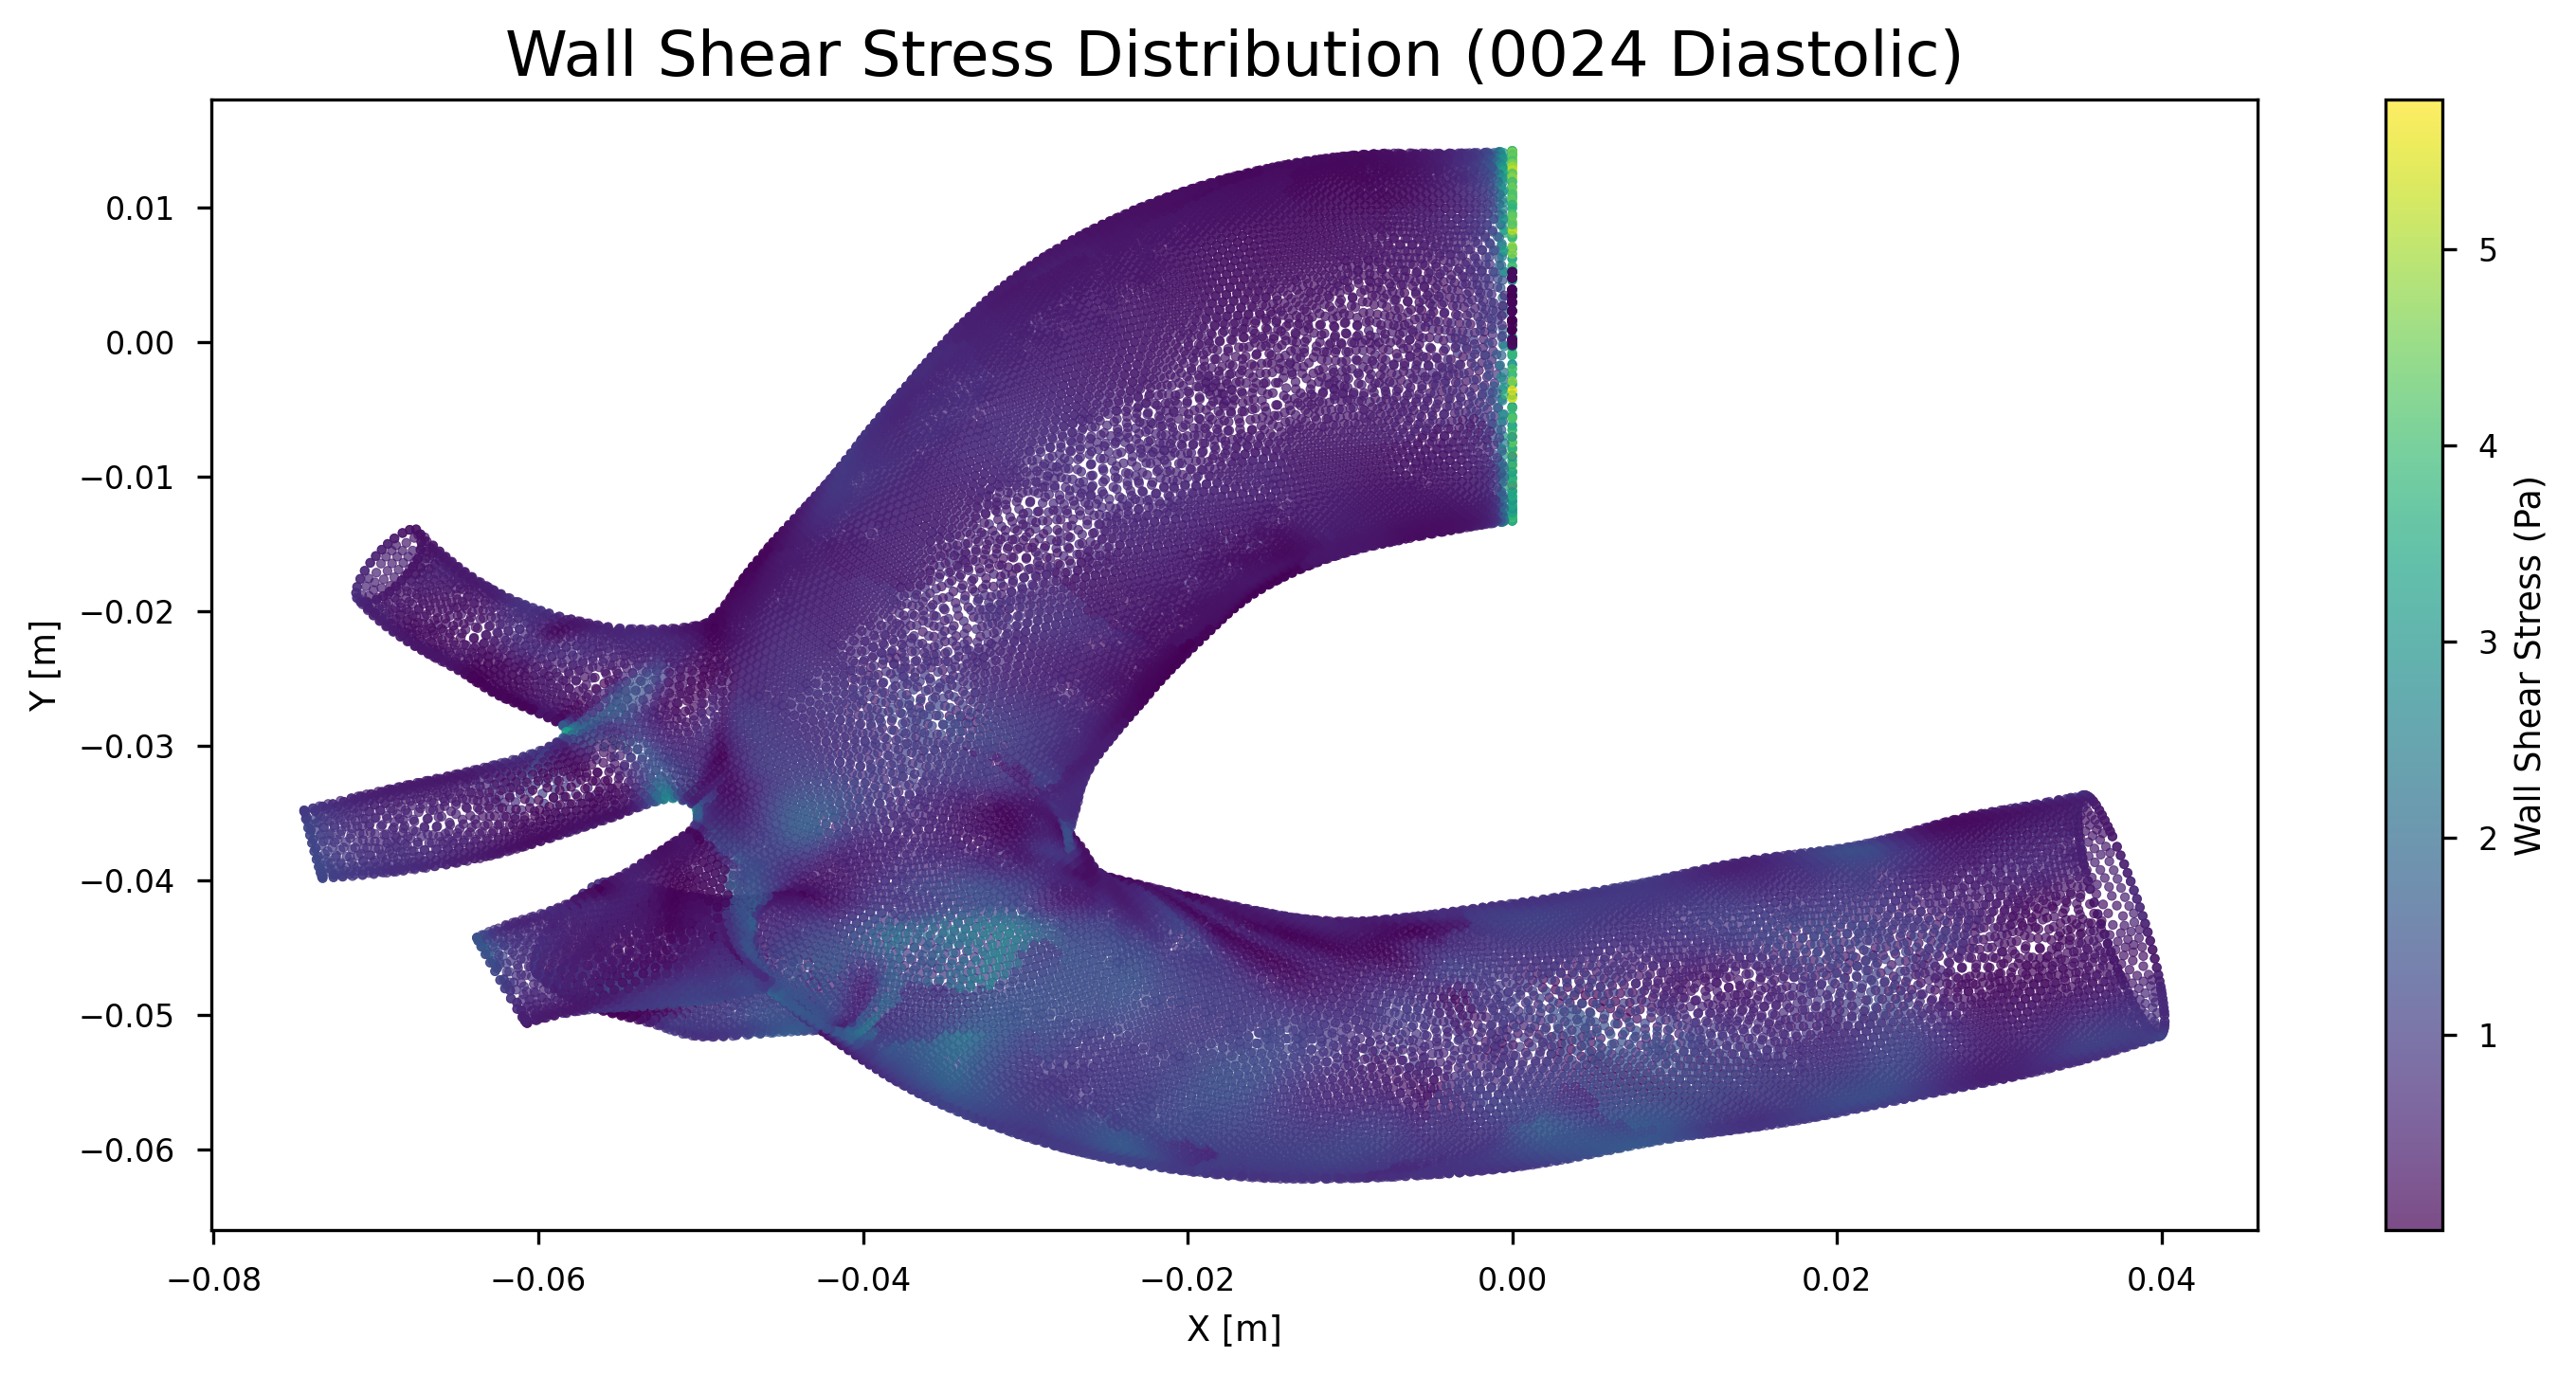
\includegraphics[width=0.9\textwidth]{0024_diastolic/wss_magnitude_distribution_0024_diastolic.png}
    \caption{2D projections (XY, XZ, YZ) of the training points, demonstrating uniform spatial coverage.}
    \label{fig:mesh_analysis}
\end{figure}

\begin{figure}[htbp]
    \centering
    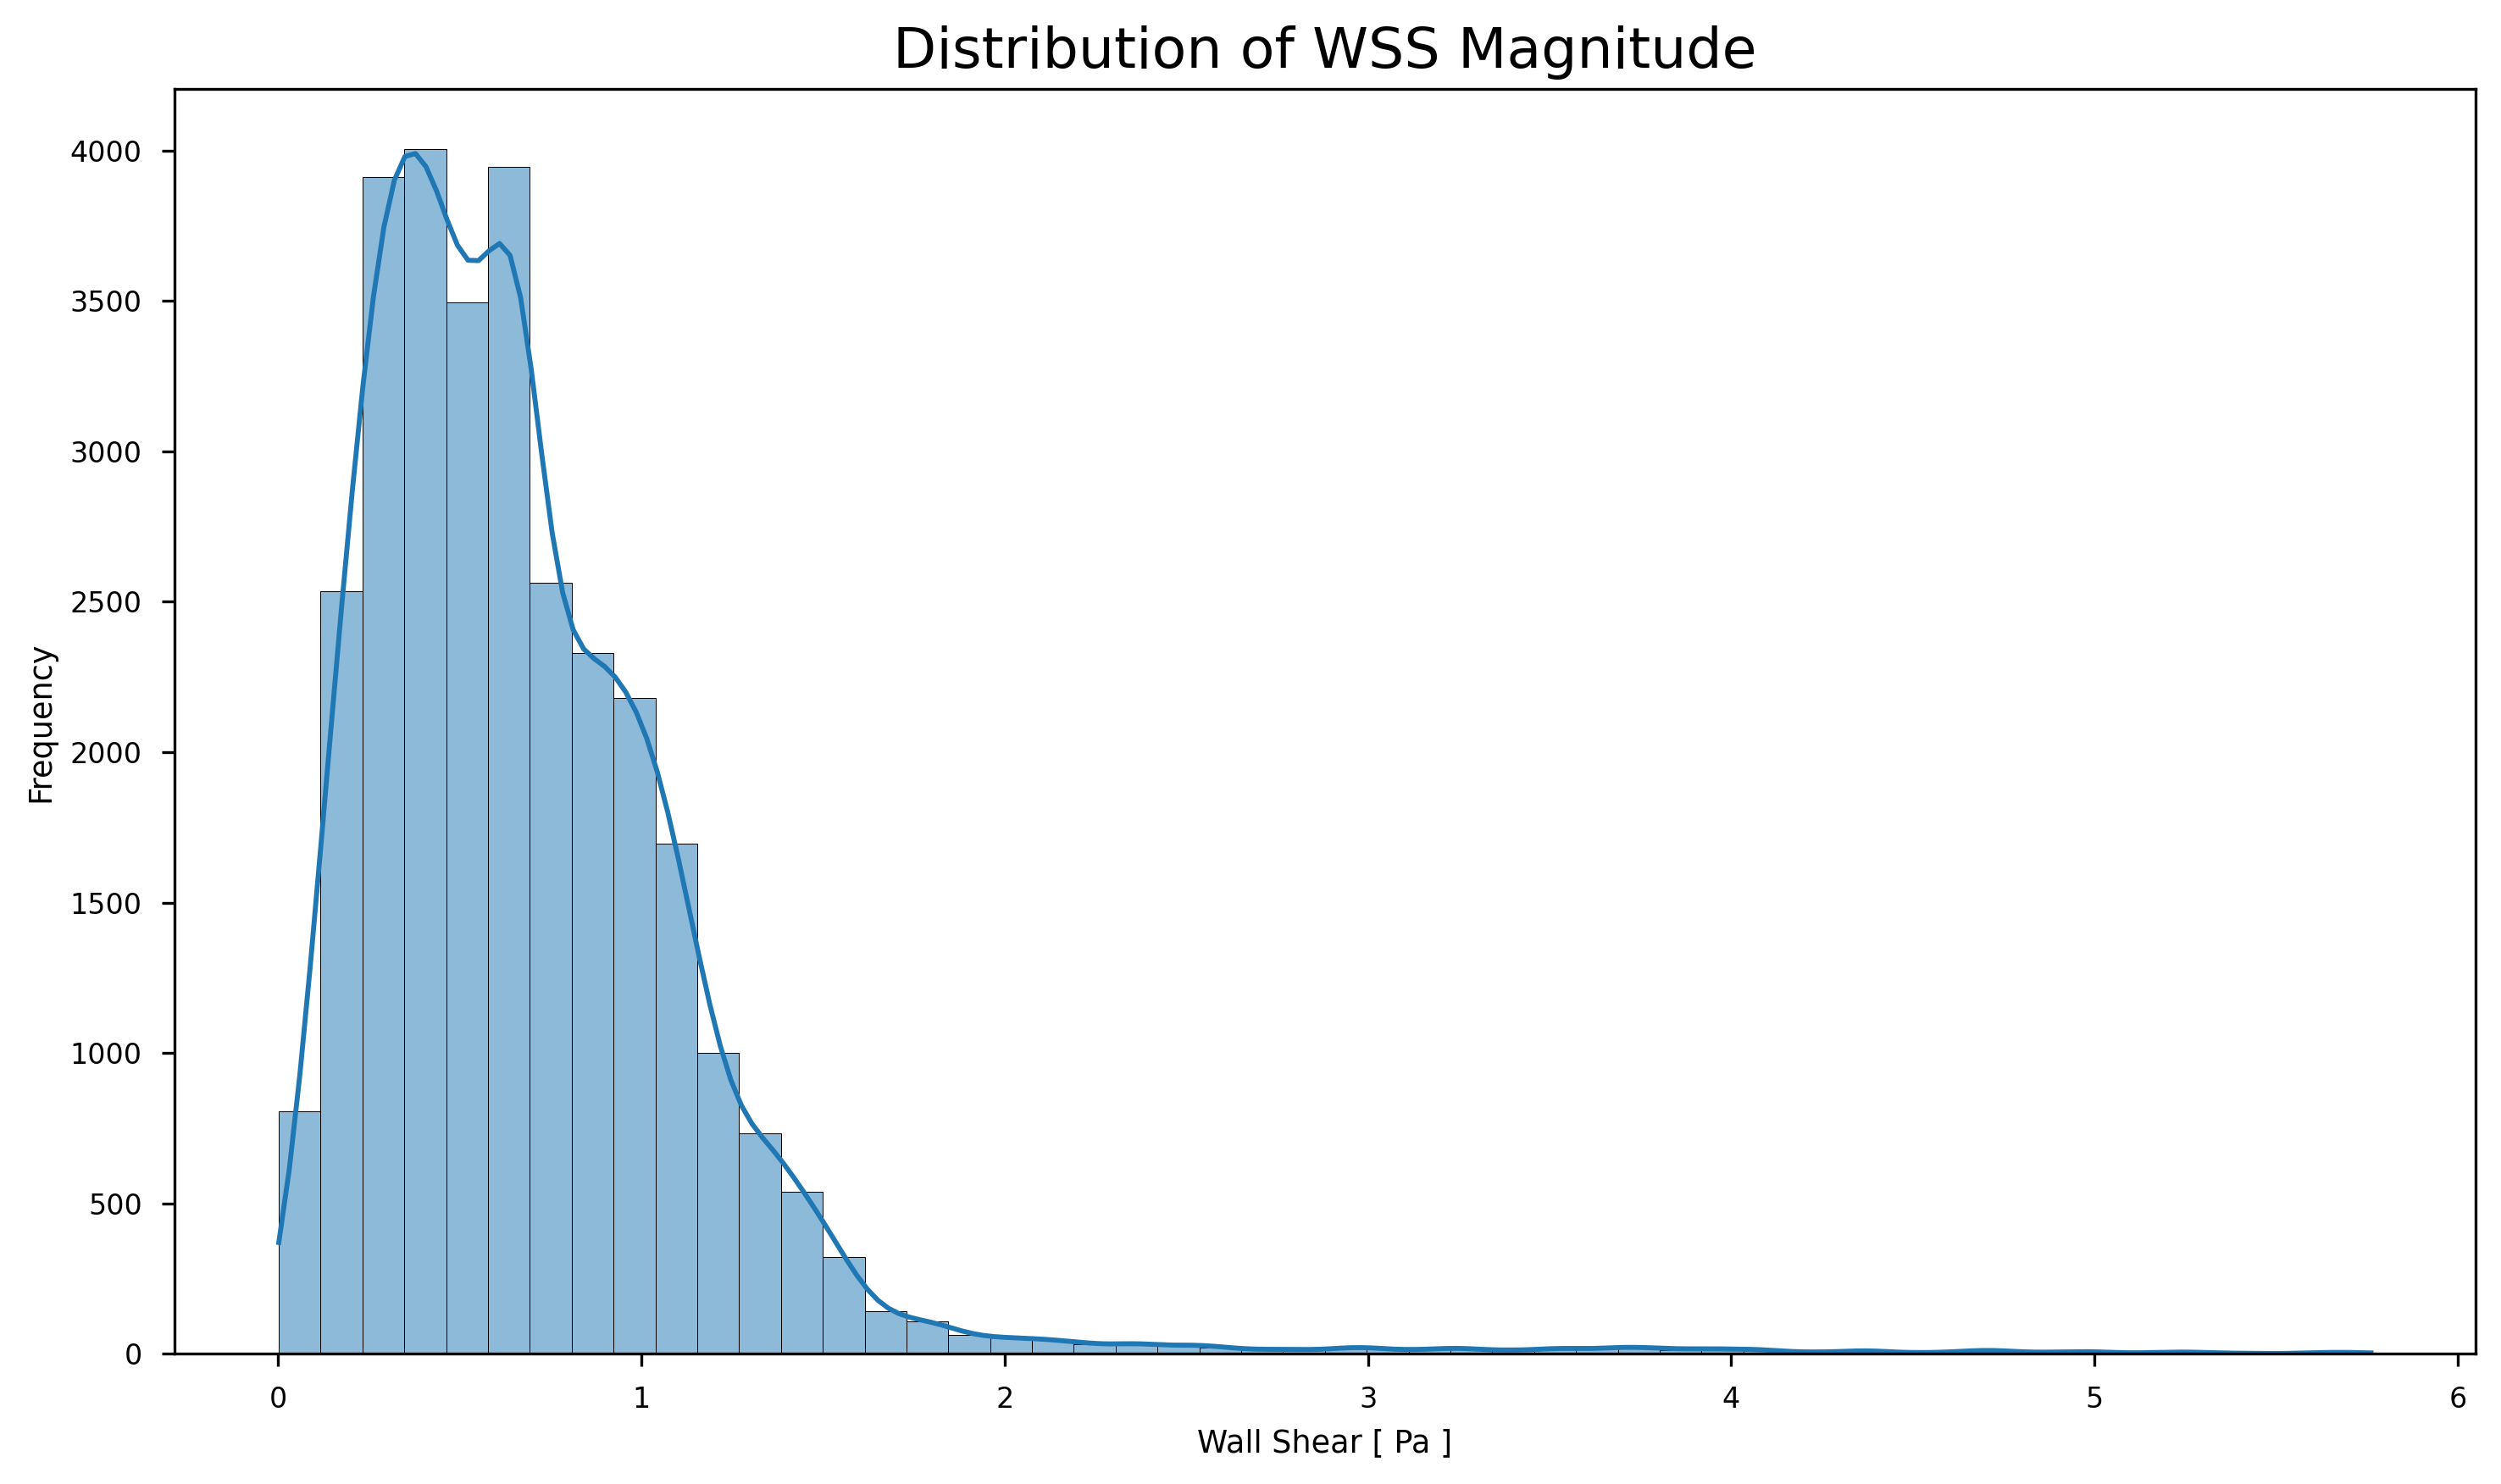
\includegraphics[width=0.9\textwidth]{0024_diastolic/pressure_distribution_0024_diastolic.png}
    \caption{Comparison between CFD data points and PINN predictions. (a) Original CFD distribution, (b) enhanced PINN prediction density, and (c) computational time comparison.}
    \label{fig:density_comparison}
\end{figure}

\subsection{Training of the PINNs}
The PINN framework was implemented in \texttt{Python} using \texttt{PyTorch}~\citep{paszke2019pytorch} and trained on a high-performance computing cluster with NVIDIA RTX8000 GPUs. The spatiotemporal data points $(x_j, y_j, z_j, t_j)$ were randomly sampled from the CFD datasets and normalized as described above. The networks were trained using the AdamW optimizer~\citep{loshchilov2017decoupled} with an initial learning rate of $1 \times 10^{-4}$, weight decay of $1 \times 10^{-4}$, and momentum parameters $(0.9, 0.999)$. A StepLR scheduler reduced the learning rate by a factor of 0.9 every 200 epochs. Training employed mixed-precision arithmetic~\citep{micikevicius2017mixed} and gradient clipping (maximum norm 1.0) for stability, and was terminated early if the validation loss did not improve for 5 consecutive epochs, with a maximum of 1000 epochs.

\subsection{Relevance to Aneurysm Studies}
PINNs offer a rapid, mesh-free alternative to full CFD simulations, particularly when boundary conditions or geometries are modified. This is of considerable clinical interest for Marfan Syndrome aortic aneurysms, where the ability to quickly explore a range of inflow profiles, wall properties, and geometrical variations can significantly enhance diagnostic and treatment planning. By maintaining the governing physics while enabling high-resolution predictions, PINNs facilitate real-time assessments and efficient sensitivity analyses, making them a promising tool for personalized vascular evaluations.

\vspace{2em}
\noindent\textbf{Note:} All code and numerical experiments for the PINN-based aneurysm flow analyses were implemented using \texttt{Python} and \texttt{PyTorch}. The self-adaptive weighting and physics-based PDE residuals were integrated into the backpropagation routine, ensuring reproducibility and transparency of the results.

\subsection{Results}
\label{sec:PINN_Results}
The PINN-based simulations were validated against benchmark CFD data for both healthy and Marfan Syndrome aortic geometries. The results demonstrate excellent agreement in velocity profiles, pressure distributions, and wall shear stress (WSS) patterns. In particular, the PINNs successfully captured complex flow phenomena such as vortex formation, flow separation, and recirculation within the aneurysm sac. The self-adaptive loss weighting mechanism effectively balanced the contributions from the physics residuals, boundary conditions, and data-fitting terms, guiding the network toward physically realistic solutions.

Figure~\ref{fig:PINN_results1} illustrates the comparison between CFD and PINN predictions for pressure and WSS in a representative Marfan Syndrome case (0021). Additionally, Figure~\ref{fig:loss_curves1} shows the evolution of the loss components over 1000 epochs, confirming stable convergence and effective balancing by the self-adaptive mechanism.

\begin{figure}[H]
    \centering
    \scriptsize
    \begin{subfigure}{0.9\textwidth}
        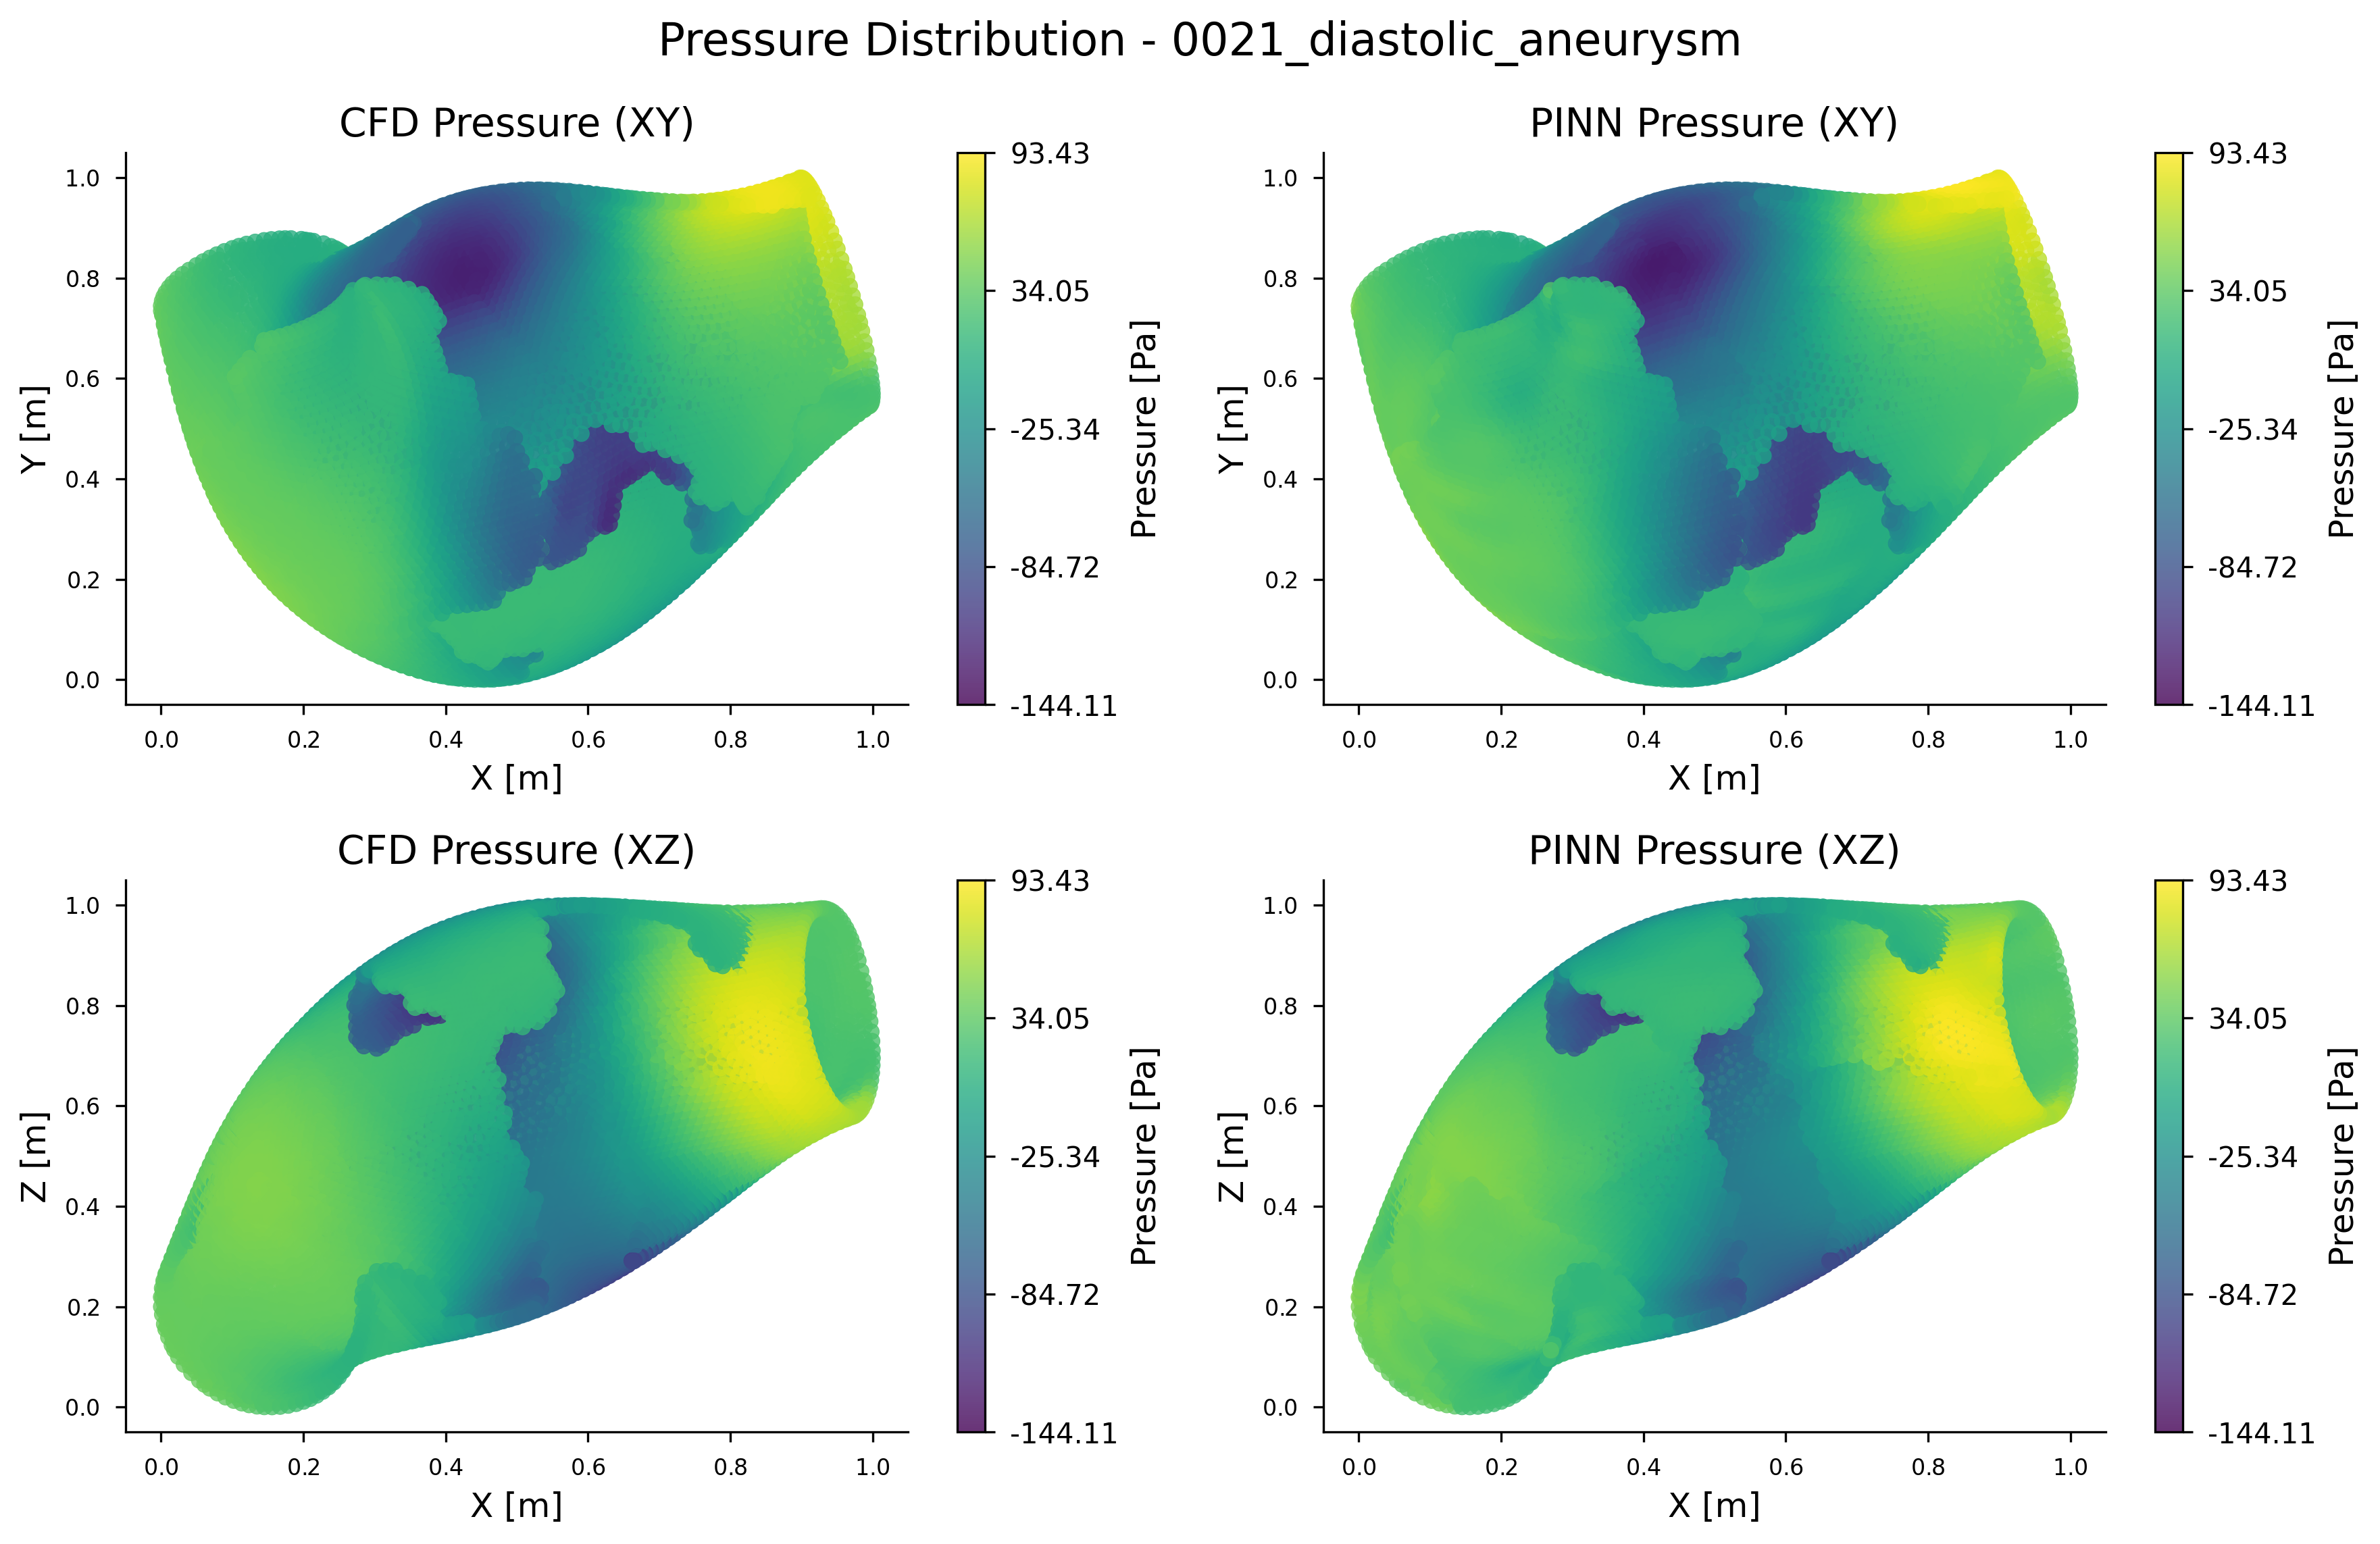
\includegraphics[width=\textwidth]{0021_diastolic_aneurysm/pressure_distribution_0021_diastolic_aneurysm.png}
        \caption{\small Pressure distribution}
    \end{subfigure}
    \begin{subfigure}{0.9\textwidth}
        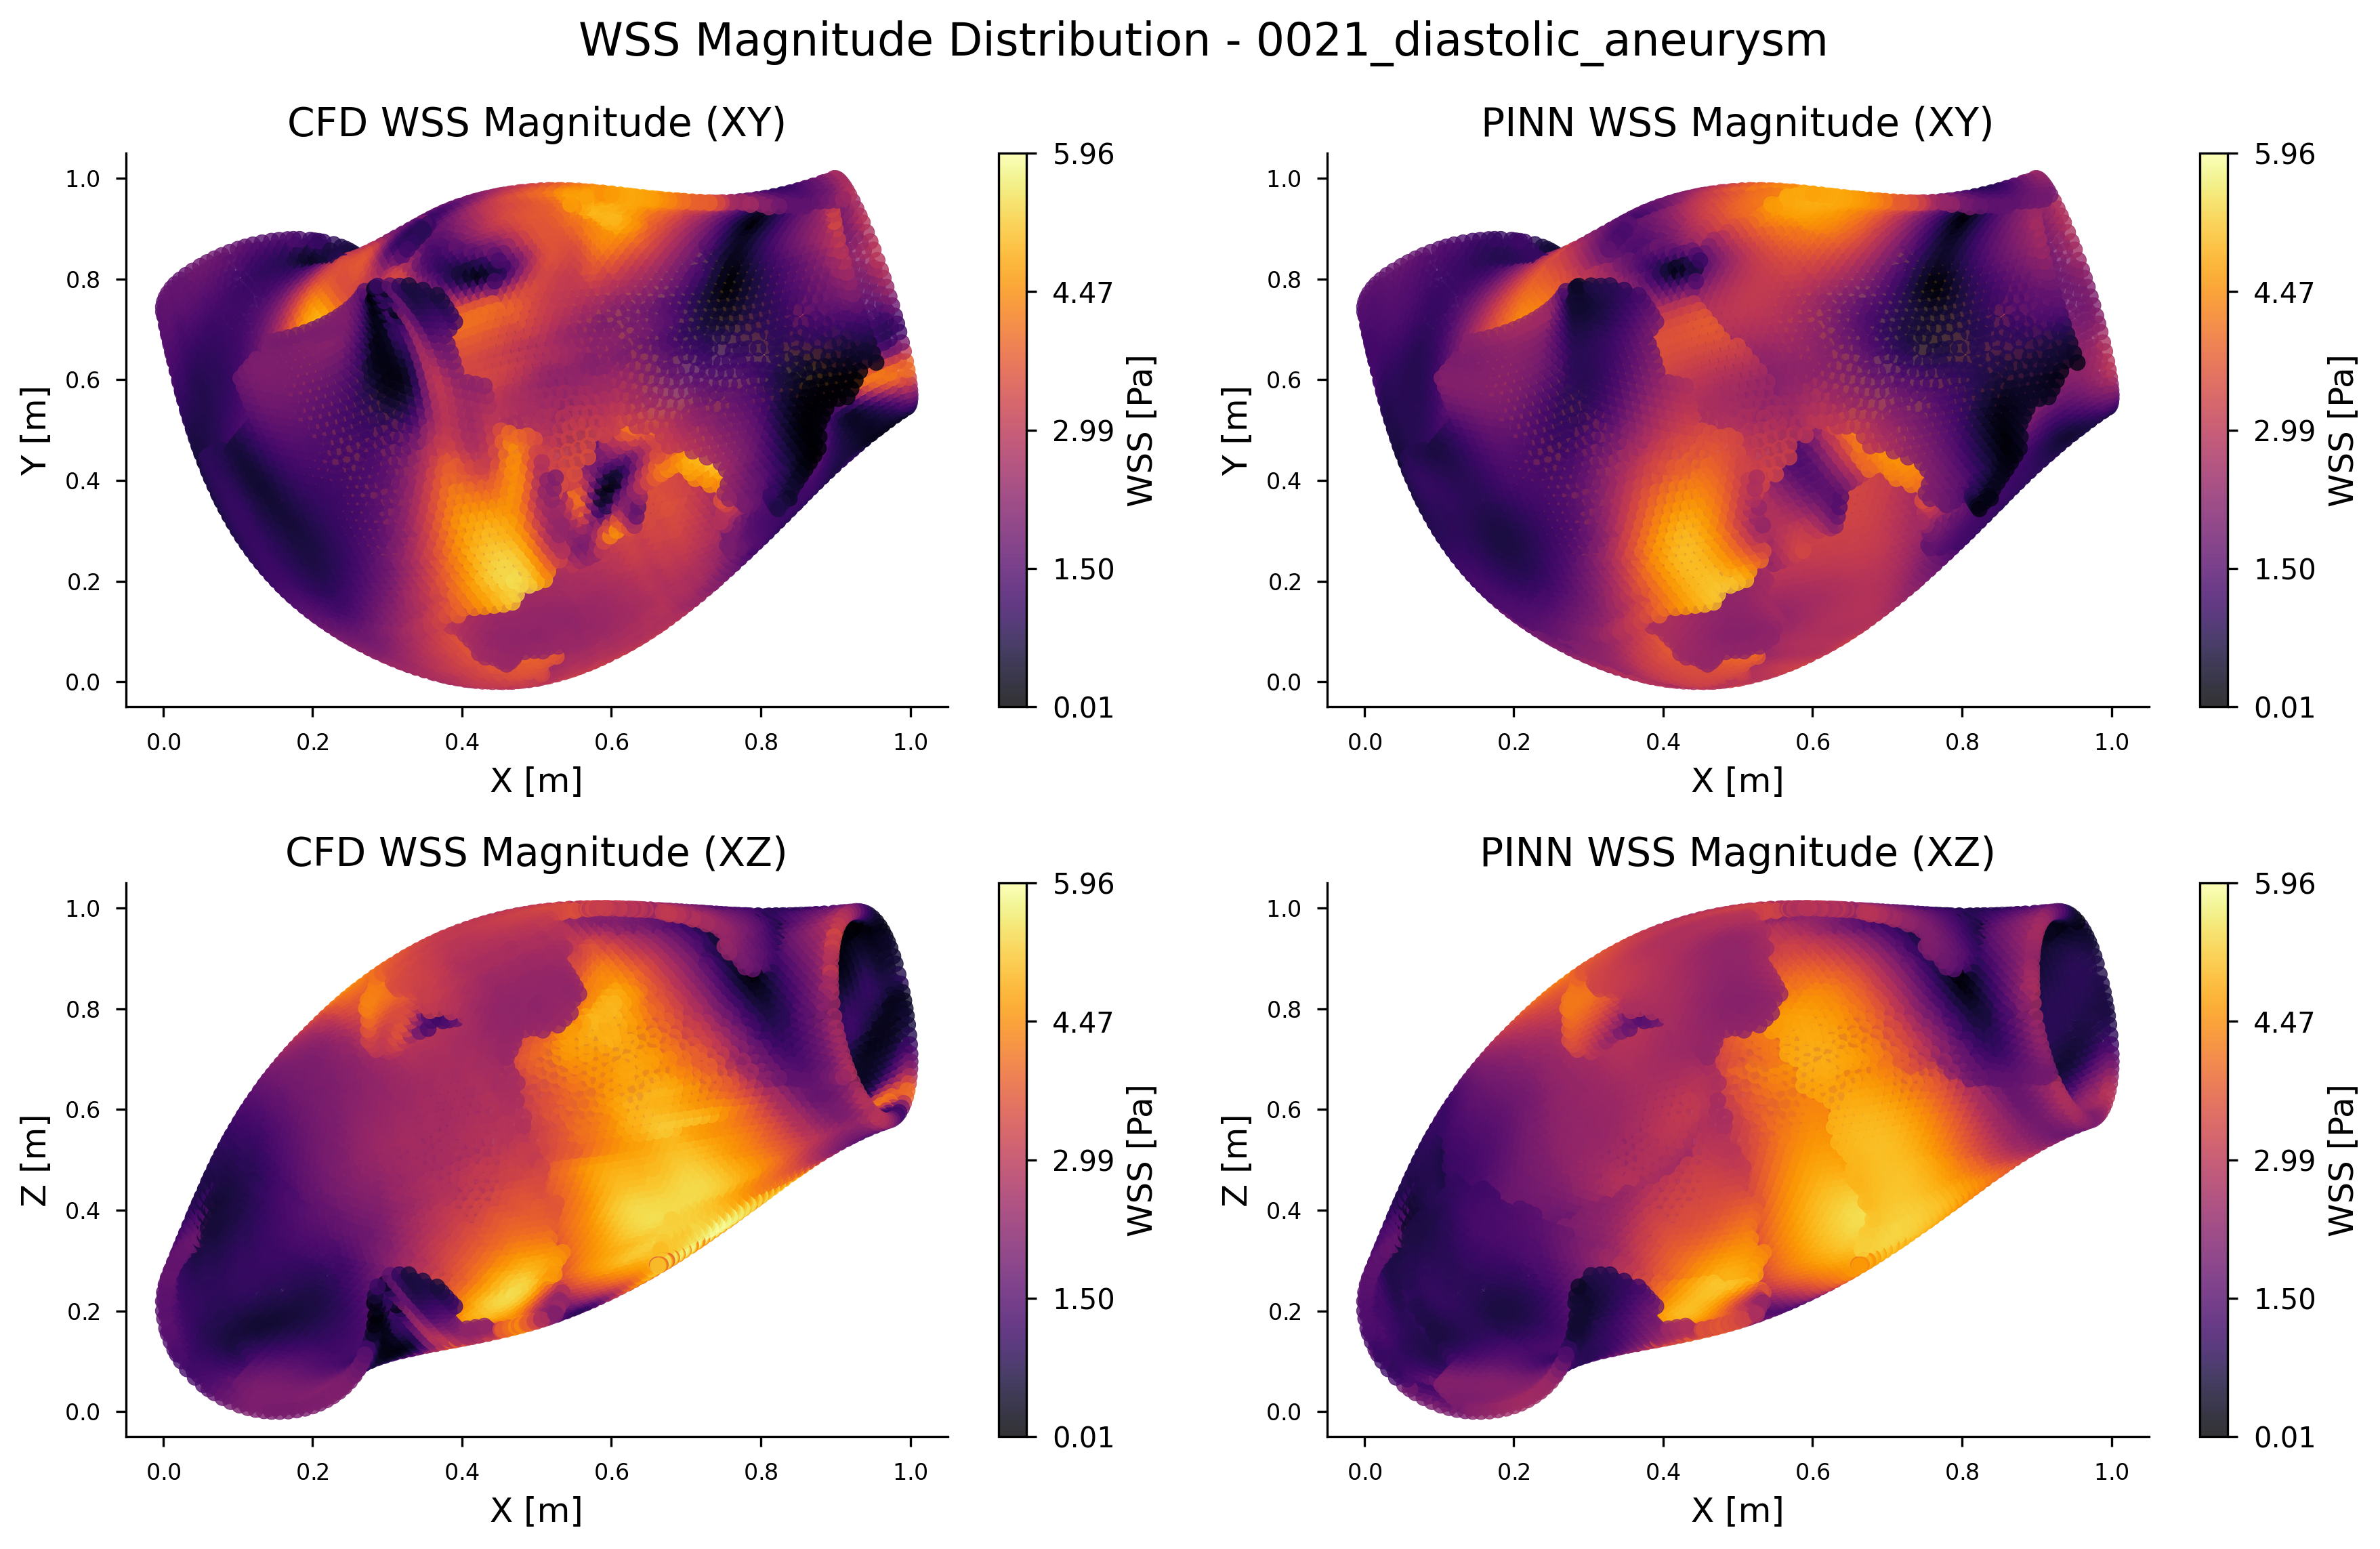
\includegraphics[width=\textwidth]{0021_diastolic_aneurysm/wss_magnitude_distribution_0021_diastolic_aneurysm.png}
        \caption{\small Wall shear stress}
    \end{subfigure}
    \caption{Comparison between CFD and PINN predictions for a Marfan Syndrome aneurysm (case 0021). The PINN accurately reproduces both the pressure field and the wall shear stress distribution.}
    \label{fig:PINN_results1}
\end{figure}

\begin{figure}[H]
    \centering
    \scriptsize
    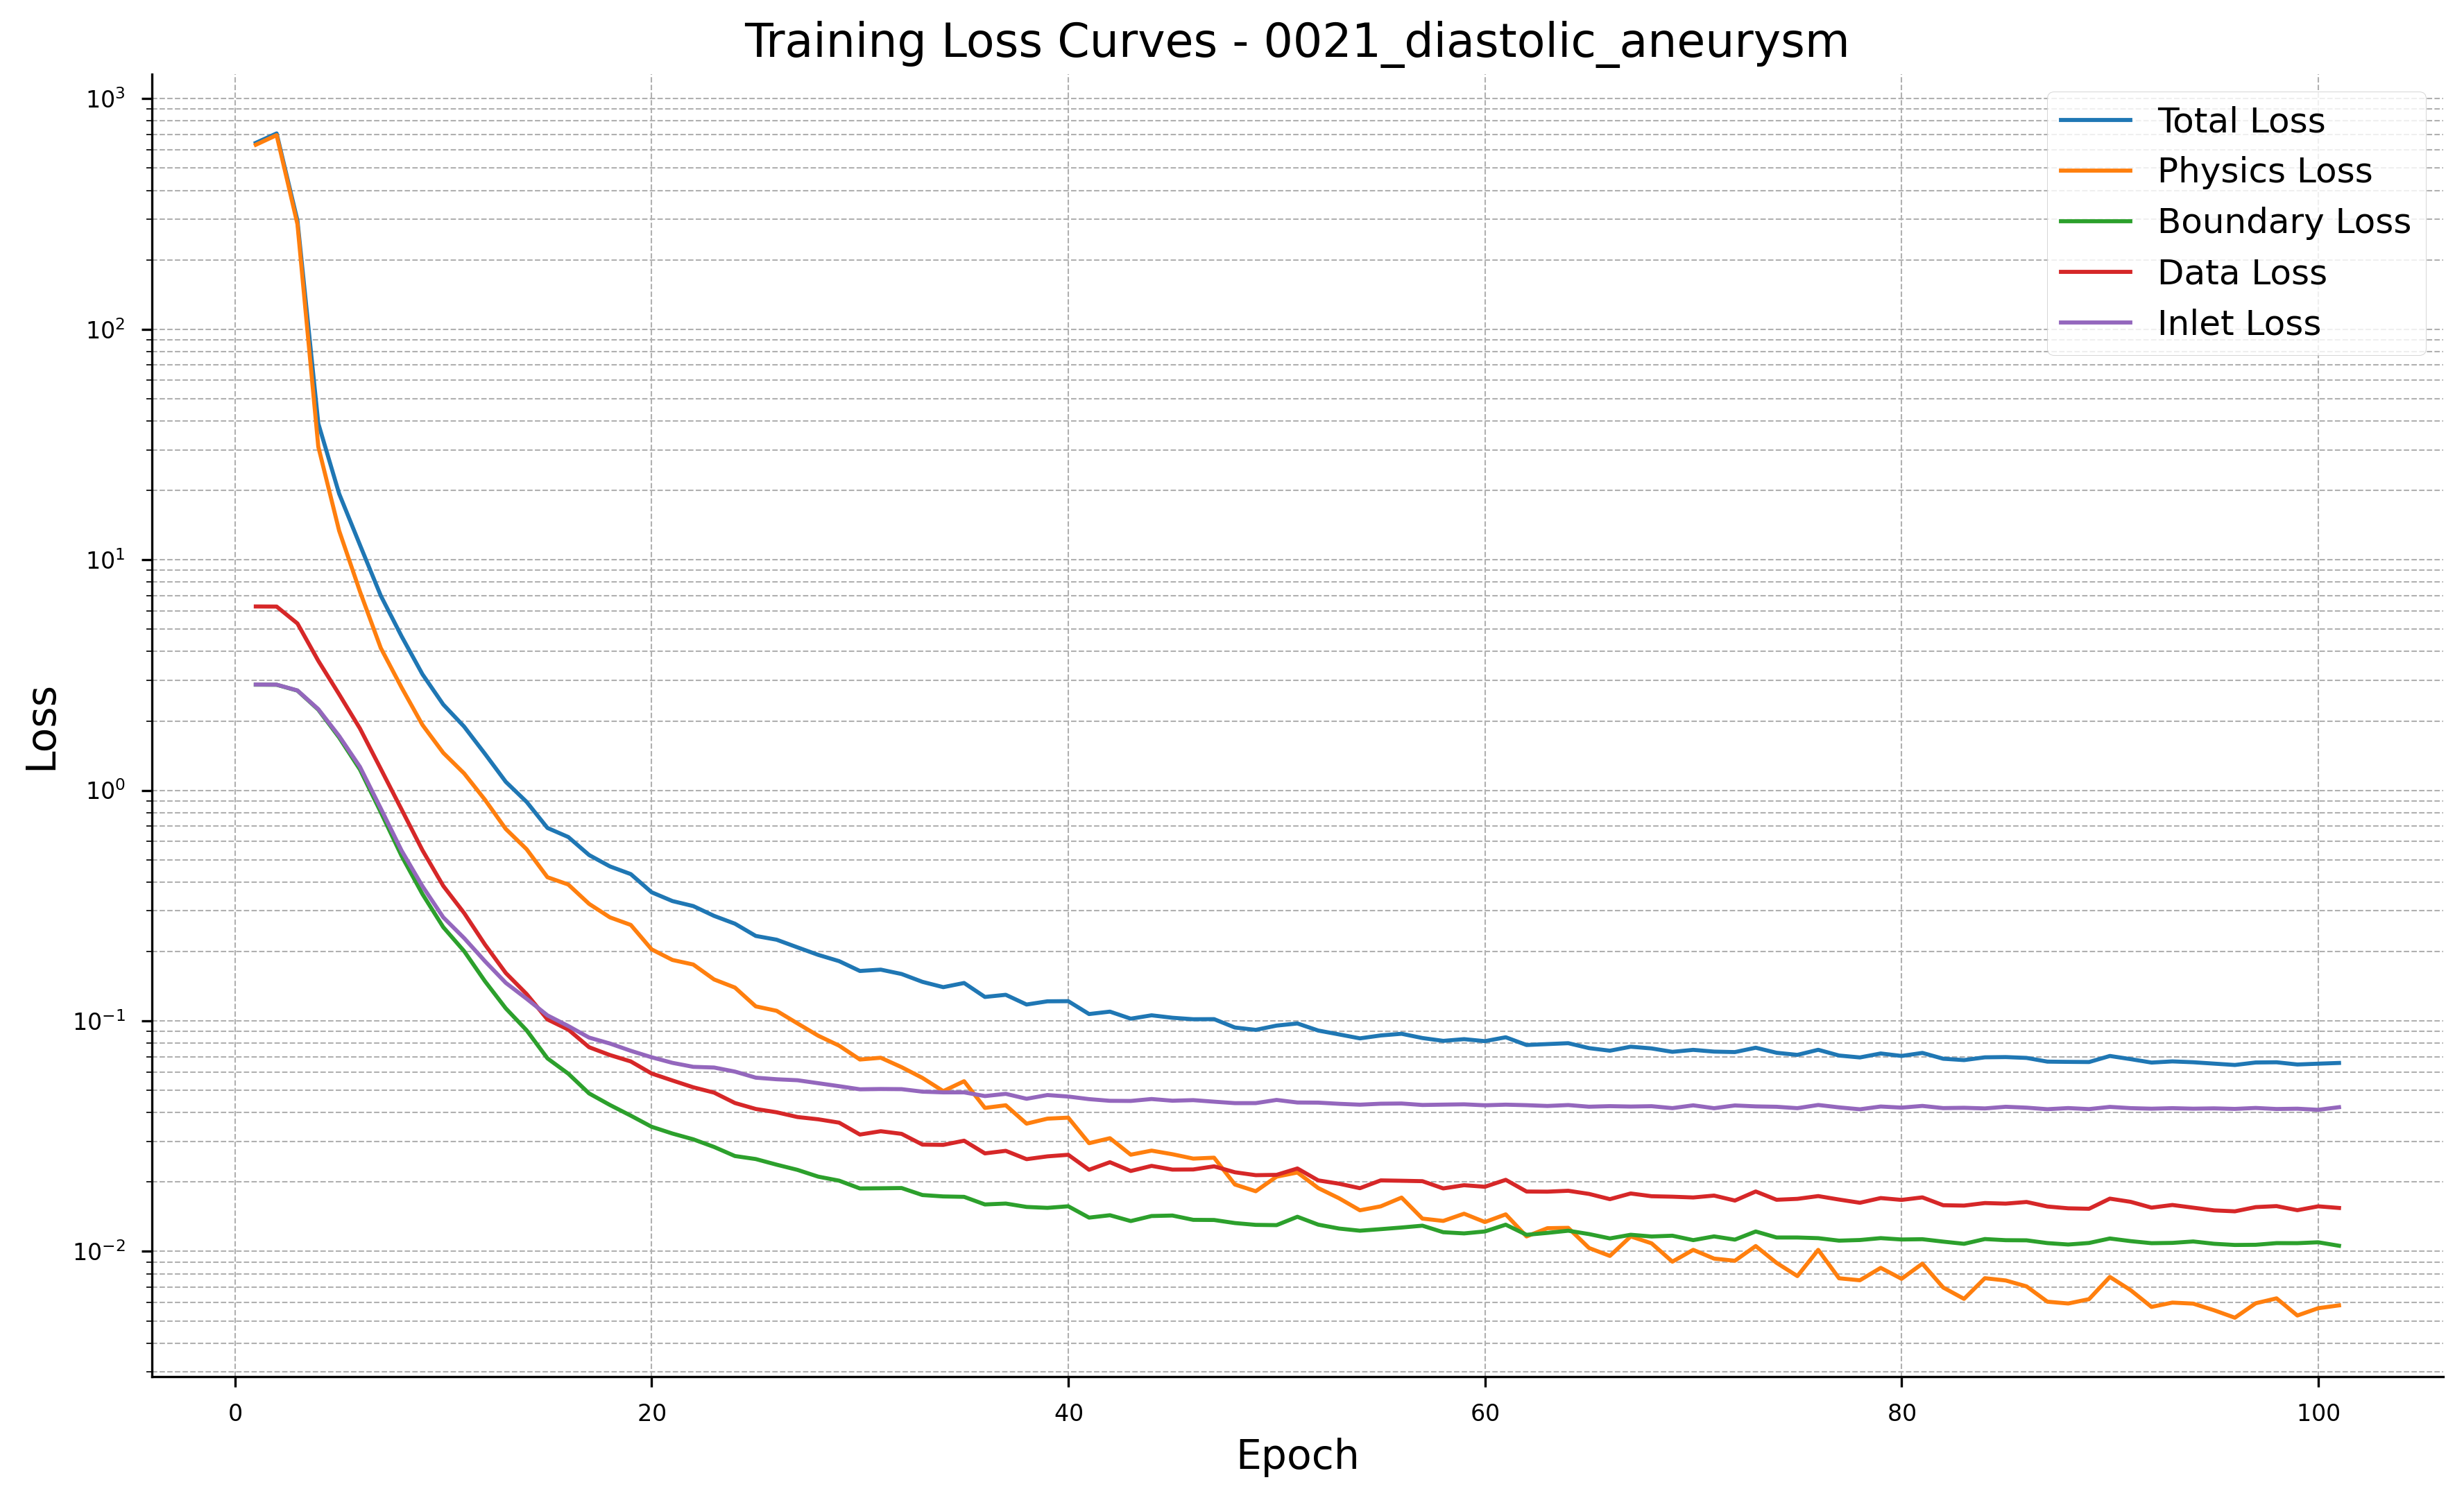
\includegraphics[width=0.9\textwidth]{0021_diastolic_aneurysm/0021_diastolic_aneurysm/loss_curves_0021_diastolic_aneurysm.png}
    \caption{Loss curves for the PINN training process, showing the evolution of the physics, boundary, inlet, and data-fitting losses over 1000 epochs. The self-adaptive loss weighting mechanism ensures balanced convergence.}
    \label{fig:loss_curves1}
\end{figure}

\bibliographystyle{unsrtnat}
\bibliography{references}

\end{document}
